% Standard pen-and-paper worksheet preamble.
% Compile with: xelatex -interaction=nonstopmode exercise.tex   (run twice)
\documentclass[a4paper, 14pt]{extarticle}
\usepackage[top=1in, bottom=1in, left=1in, right=1in]{geometry}
\usepackage{amsmath}
\usepackage{amssymb}
\usepackage{graphicx}
\usepackage{hyperref}
\usepackage{tcolorbox}
\usepackage{enumitem}
\usepackage{multicol}
\usepackage{etoolbox}
\usepackage{tikz}
\usepackage{fontspec}
\usetikzlibrary{calc,decorations,patterns,arrows,decorations.pathmorphing,positioning}
\definecolor{pltblue}{HTML}{1F77B4}

% Handwriting font, resolved once into \ppfont and \ppfontname.
%
% "Pretty Neat" (xkcd-style) is the house face and is installed on almost
% nothing. Excalifont is vendored in tools/fonts/ and installed by CI, so it is
% the one face that is always present; Latin Modern is the last resort.
%
% Naming a font that is not installed is a hard error, not a fallback, which is
% why this is a chain and not a line: seven sheets used to name one outright
% and stopped building the day it was uninstalled.
\def\ppfontname{Latin Modern Roman}
\IfFontExistsTF{Pretty Neat}{\def\ppfontname{Pretty Neat}}{%
  \IfFontExistsTF{Humor Sans}{\def\ppfontname{Humor Sans}}{%
    \IfFontExistsTF{Excalifont}{\def\ppfontname{Excalifont}}{}}}
\expandafter\newfontfamily\expandafter\ppfont\expandafter{\ppfontname}
\expandafter\setmainfont\expandafter{\ppfontname}
\tikzset{every picture/.style={/utils/exec={\ppfont}}}
\AtBeginEnvironment{tabular}{\ppfont}

% xkcd-style hand-drawn line decoration.
% WARNING: applying [xkcd] to many nodes can throw "Dimension too large".
% Use it on a handful of \draw lines only, never on every node.
\makeatletter
\pgfset{
  /pgf/decoration/randomness/.initial=2,
  /pgf/decoration/wavelength/.initial=100
}
\pgfdeclaredecoration{sketch}{init}{
  \state{init}[width=0pt,next state=draw,persistent precomputation={
    \pgfmathsetmacro\pgf@lib@dec@sketch@t0
  }]{}
  \state{draw}[width=\pgfdecorationsegmentlength,
  auto corner on length=\pgfdecorationsegmentlength,
  persistent precomputation={
    \pgfmathsetmacro\pgf@lib@dec@sketch@t{mod(\pgf@lib@dec@sketch@t+pow(\pgfkeysvalueof{/pgf/decoration/randomness},rand),\pgfkeysvalueof{/pgf/decoration/wavelength})}
  }]{
    \pgfmathparse{sin(2*\pgf@lib@dec@sketch@t*pi/\pgfkeysvalueof{/pgf/decoration/wavelength} r)}
    \pgfpathlineto{\pgfqpoint{\pgfdecorationsegmentlength}{\pgfmathresult\pgfdecorationsegmentamplitude}}
  }
  \state{final}{}
}
\tikzset{xkcd/.style={decorate,decoration={sketch,segment length=0.5pt,amplitude=0.5pt}}}
\makeatother

\setlength{\parindent}{0pt}
\setlength{\parskip}{0.5em}

\begin{document}

\section*{\ppfont Who's the Big Cheese in the University Clubs?}

You're new at a university and want to understand the social dynamics of the
students. Here's the club membership information:

\begin{center}
\begin{tabular}{|l|l|}
    \hline
    \textbf{Club} & \textbf{Members} \\
    \hline
    Drama Club & Sarah, Mike, Emma \\
    Art Club & Emma, Alex \\
    Volunteer Club & Alex, Olivia, James \\
    Sailing Club & Alex, Sophia \\
    Chess Club & Sophia, Ethan, Ava, Noah \\
    Debate Team & Noah, Lily \\
    Math Club & Noah, Lucas \\
    Tennis Club & Noah, Henry \\
    \hline
\end{tabular}
\end{center}

{\bf Question 1}:
Draw a network where students are nodes, and two students are joined by an edge
whenever they are in the same club.

\clearpage

{\bf Question 2}:
Without doing any calculations, which student would you approach first if you
wanted to spread information quickly about a new inter-club event? Explain your
reasoning.

\vspace{9em}

{\bf Question 3}:
Without doing any calculations, which student would you recommend as ``Club
Coordinator'', whose job is to help the different clubs talk to each other?
Explain your reasoning.

\vspace{9em}

Keep both answers where you can see them. You will be asked for them again at
the end, once you have some numbers.

\clearpage

Here is that network drawn out. Check it against the one you drew --- if they
differ, find the club you missed.

\begin{center}
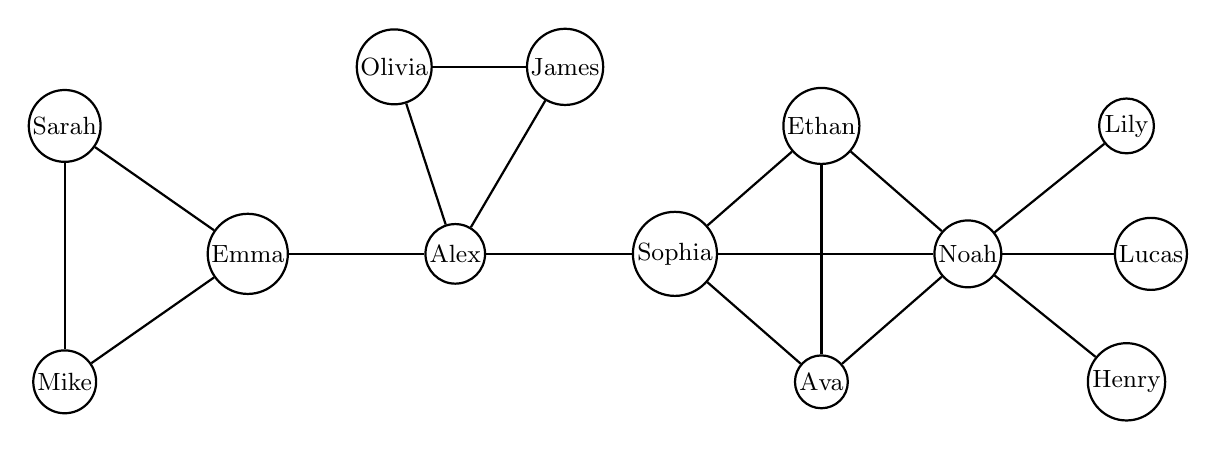
\begin{tikzpicture}[x=1.55cm, y=1.25cm, thick,
                    every node/.style={draw, circle, inner sep=0.8pt,
                                       font=\small, fill=white}]
    \node (Sarah)  at (0,    1.3)  {Sarah};
    \node (Mike)   at (0,   -1.3)  {Mike};
    \node (Emma)   at (1.5,  0)    {Emma};
    \node (Olivia) at (2.7,  1.9)  {Olivia};
    \node (James)  at (4.1,  1.9)  {James};
    \node (Alex)   at (3.2,  0)    {Alex};
    \node (Sophia) at (5.0,  0)    {Sophia};
    \node (Ethan)  at (6.2,  1.3)  {Ethan};
    \node (Ava)    at (6.2, -1.3)  {Ava};
    \node (Noah)   at (7.4,  0)    {Noah};
    \node (Lily)   at (8.7,  1.3)  {Lily};
    \node (Lucas)  at (8.9,  0)    {Lucas};
    \node (Henry)  at (8.7, -1.3)  {Henry};

    \draw (Sarah) -- (Mike);
    \draw (Sarah) -- (Emma);
    \draw (Mike) -- (Emma);
    \draw (Emma) -- (Alex);
    \draw (Alex) -- (Olivia);
    \draw (Alex) -- (James);
    \draw (Olivia) -- (James);
    \draw (Alex) -- (Sophia);
    \draw (Sophia) -- (Ethan);
    \draw (Sophia) -- (Ava);
    \draw (Sophia) -- (Noah);
    \draw (Ethan) -- (Ava);
    \draw (Ethan) -- (Noah);
    \draw (Ava) -- (Noah);
    \draw (Noah) -- (Lily);
    \draw (Noah) -- (Lucas);
    \draw (Noah) -- (Henry);
\end{tikzpicture}
\end{center}

{\bf Question 4}: {\bf Count the friends.} For each student, count how many
other students they are joined to. Who has the most?

\begin{center}
{\setlength{\tabcolsep}{5pt}
\begin{tabular}{|l|p{1.6cm}|l|p{1.6cm}|}
\hline
\textbf{Student} & \textbf{friends} & \textbf{Student} & \textbf{friends} \\
\hline
Sarah  & & Ethan & \\[0.35cm] \hline
Mike   & & Ava   & \\[0.35cm] \hline
Emma   & & Noah  & \\[0.35cm] \hline
Alex   & & Lily  & \\[0.35cm] \hline
Olivia & & Lucas & \\[0.35cm] \hline
James  & & Henry & \\[0.35cm] \hline
Sophia & &       & \\[0.35cm] \hline
\end{tabular}}
\end{center}

Winner: \underline{\hspace{5cm}}

\clearpage

Take the {\bf three} students who came top in Question 4. They are your
candidates for the rest of the sheet. Write their names in the tables below.

{\bf Question 5}: {\bf How far is everyone?} For each candidate, count the
number of steps along edges to every other student --- the shortest route, not
just any route. A candidate's distance to themself is 0, so each row has twelve
numbers that count: add them and divide by twelve. Who is closest to everybody?

\begin{center}
{\setlength{\tabcolsep}{3pt}
\begin{tabular}{|p{1.9cm}|*{13}{p{0.5cm}|}p{1.1cm}|}
\hline
 & Sa & Mi & Em & Al & Ol & Ja & So & Et & Av & No & Li & Lu & He & \textbf{avg} \\
\hline
 & & & & & & & & & & & & & & \\[0.75cm] \hline
 & & & & & & & & & & & & & & \\[0.75cm] \hline
 & & & & & & & & & & & & & & \\[0.75cm] \hline
\end{tabular}}
\end{center}

{\footnotesize Sa Sarah \quad Mi Mike \quad Em Emma \quad Al Alex \quad
Ol Olivia \quad Ja James \quad So Sophia \quad Et Ethan \quad Av Ava \quad
No Noah \quad Li Lily \quad Lu Lucas \quad He Henry}

Winner: \underline{\hspace{5cm}}

\vspace{1em}

{\bf Question 6}: {\bf Who is indispensable?} Put your thumb over one candidate
and all of their edges. Some pairs of the remaining twelve students can now not
reach each other \emph{at all}. Count those pairs, for each candidate in turn.

\begin{center}
{\setlength{\tabcolsep}{6pt}
\begin{tabular}{|p{3.2cm}|p{6cm}|p{2.6cm}|}
\hline
\textbf{Candidate} & \textbf{sizes of the groups left behind} & \textbf{pairs cut off} \\
\hline
 & & \\[0.7cm] \hline
 & & \\[0.7cm] \hline
 & & \\[0.7cm] \hline
\end{tabular}}
\end{center}

{\footnotesize Mechanics, not the answer: if covering someone leaves three
groups of sizes 2, 3 and 4, then the pairs cut off number
$2\times3 + 2\times4 + 3\times4 = 26$.}

Winner: \underline{\hspace{5cm}}

\clearpage

{\bf Question 7}: {\bf Pass the scores around.} Give every one of the thirteen
students one point. Now play this game: each student throws away their own
score and takes instead the {\bf sum of their friends' scores}. Play it twice.

Round 1 is quick --- you already did it in Question 4, so write that column in.
For round 2, add up the number of friends of each of your candidate's friends.

\begin{center}
{\setlength{\tabcolsep}{6pt}
\begin{tabular}{|p{3.4cm}|p{3.2cm}|p{6cm}|}
\hline
\textbf{Candidate} & \textbf{after round 1} & \textbf{after round 2} \\
\hline
 & & \\[0.9cm] \hline
 & & \\[0.9cm] \hline
 & & \\[0.9cm] \hline
\end{tabular}}
\end{center}

Winner: \underline{\hspace{5cm}}

\vspace{1.5em}

{\bf Question 8}: {\bf The point of the whole sheet.} Copy your four winners
into the four boxes.

\begin{center}
{\setlength{\tabcolsep}{5pt}
\begin{tabular}{|p{6.5cm}|p{6cm}|}
\hline
most friends (Q4) & \\[0.6cm] \hline
shortest average distance (Q5) & \\[0.6cm] \hline
most pairs cut off (Q6) & \\[0.6cm] \hline
highest score after two rounds (Q7) & \\[0.6cm] \hline
\end{tabular}}
\end{center}

How many \emph{different} names did you write?
\underline{\hspace{2cm}}

\clearpage

Nothing about the network changed between those four boxes. Only the question
did. Write one sentence for each box saying what question it was really asking
about a student.

\vspace{11em}

{\bf Question 9}: Now name a situation --- a real one, at a real university ---
in which each of your winners would be the right person to pick, and the others
would be the wrong choice.

\vspace{11em}

\clearpage

{\bf Question 10}: Go back to Questions 2 and 3. With the numbers in front of
you, do you still give the same two names? Which of your four measures matches
the question ``who spreads news fastest?'', and which matches ``who should be
Club Coordinator?''

\vspace{11em}

{\bf Question 11}: {\bf Break it.} A Robotics Club is formed, and Noah and Emma
both join it. Add that one edge to the drawing on page 3.

Redo Question 6 in your head for each candidate. One of them goes from being
indispensable to being dispensable --- who, and why? Does that person still lie
on plenty of the shortest routes, even so?

\vspace{11em}

\clearpage

{\bf Question 12}: In Question 7 you played two rounds of passing scores. You
don't need to do the calculation --- just describe the recipe you would hand to
a computer so that it could keep playing that game forever, on a network of a
million students. What happens to the size of the numbers as the rounds go by,
and what would you have to do about it?

\vspace{12em}

\end{document}
